\documentclass[12pt]{article}
\usepackage[utf8]{inputenc}
\usepackage{upquote}
\usepackage[margin=20mm]{geometry} 
\usepackage{amsmath,amsthm,amssymb}
\usepackage{graphicx}
\usepackage{listings}
\newenvironment{statement}[2][Statement]{\begin{trivlist}
\item[\hskip \labelsep {\bfseries #1}\hskip \labelsep {\bfseries #2.}]}{\end{trivlist}}
\usepackage{xcolor}

\usepackage{subfigure}


% Listings package for code rendering (No external dependencies)
\usepackage{listings}  
\usepackage{xcolor}   % Color support
\usepackage{tcolorbox} % Box for better appearance

% Define custom colors for code highlighting
\definecolor{codegreen}{rgb}{0,0.6,0}
\definecolor{codegray}{rgb}{0.5,0.5,0.5}
\definecolor{codepurple}{rgb}{0.58,0,0.82}
\definecolor{backcolour}{rgb}{0.95,0.95,0.92}


\lstset{frame=tb,
    language=Python,
    backgroundcolor=\color{backcolour},   
    commentstyle=\color{codegreen},
    keywordstyle=\color{magenta},
    numberstyle=\tiny\color{codegray},
    stringstyle=\color{codepurple},
    basicstyle=\ttfamily\footnotesize,
    breakatwhitespace=false,         
    breaklines=true,                 
    keepspaces=true,                 
    numbers=left,       
    numbersep=5pt,                  
    showspaces=false,                
    showstringspaces=false,
    showtabs=false,                  
    tabsize=2,
}





\title{Assignment 7}


\author{Author \\
 Wanjing Hu / fng685@alumni.ku.dk  \\
 Shuangcheng Jia / bkg713@alumni.ku.dk/   \\
 Zhigao Yan / sxd343@alumni.ku.dk  \\
} 

\begin{document}
\maketitle

\section{Segmentation}
%shuangcheng
\subsection{}
\begin{figure}[ht]
    \centering
    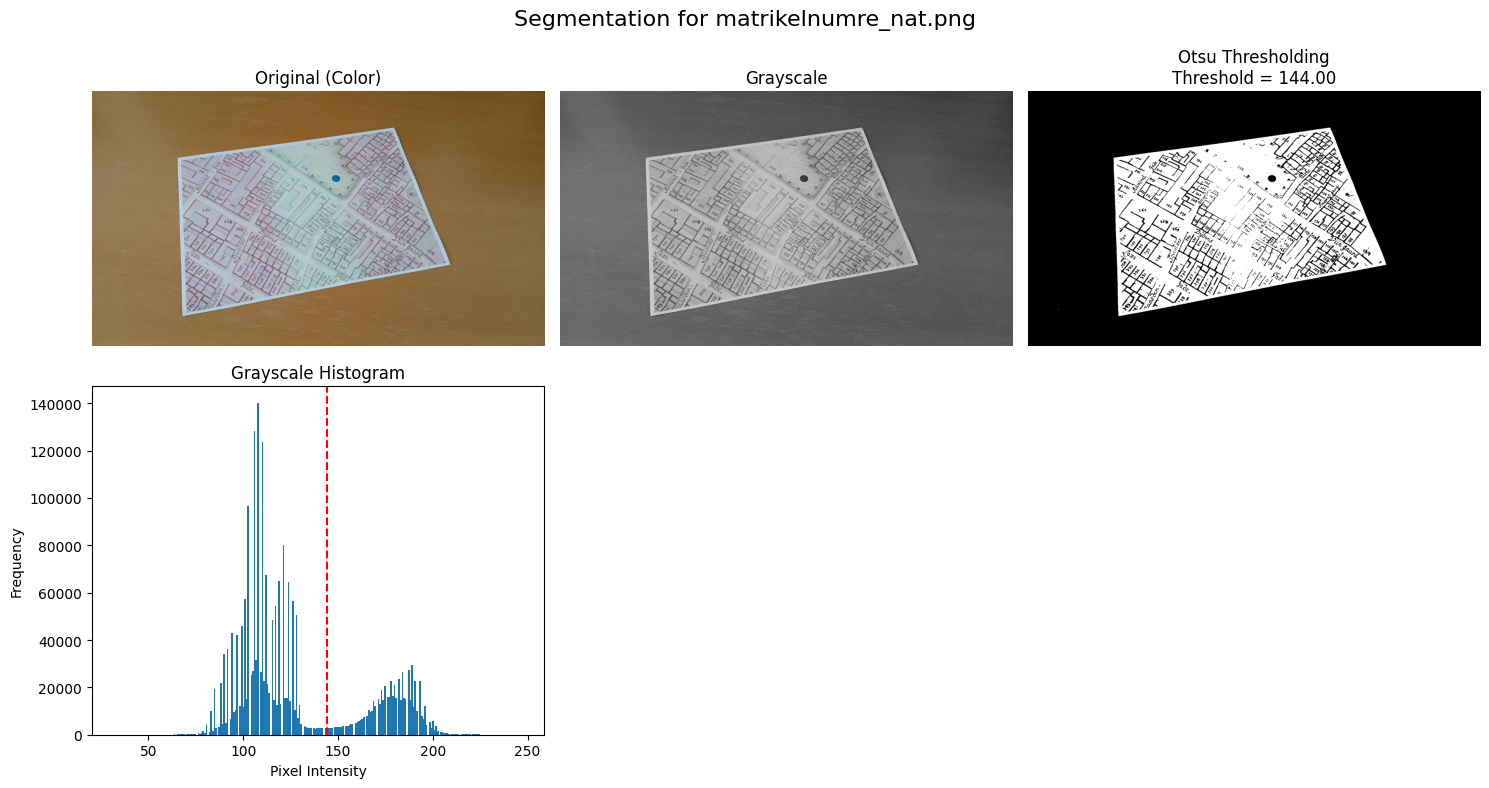
\includegraphics[width=0.7\textwidth]{pics/a7-1.1-1.png}
    \caption{Results for matrikelnumre-nat.png}
    \label{1.1-1}
\end{figure}

\begin{figure}[ht]
    \centering
    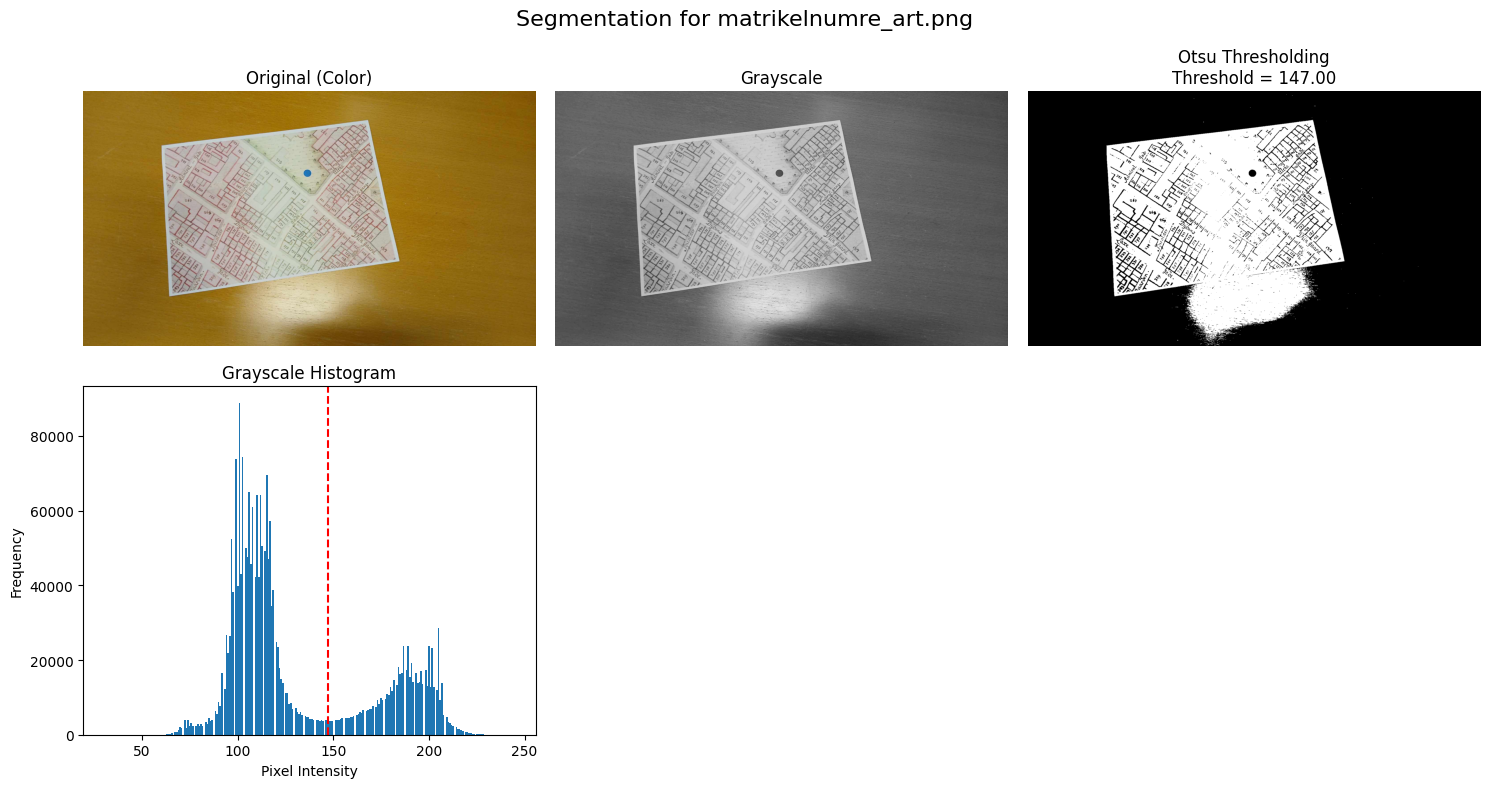
\includegraphics[width=0.7\textwidth]{pics/a7-1.1-2.png}
    \caption{Results for matrikelnumre-art.png}
    \label{1.1-2}
\end{figure}

\begin{lstlisting}
def plot_images_and_histograms(image_name):
    image_color = cv2.imread(image_name)
    image_rgb = cv2.cvtColor(image_color, cv2.COLOR_BGR2RGB)
    image_gray = cv2.cvtColor(image_color, cv2.COLOR_BGR2GRAY)

    #  Otsu  threshold
    thresh_val = threshold_otsu(image_gray)
    binary = image_gray > thresh_val

    ###The Figure code is omitted. (Including color, grayscale image display and grayscale histogram display)

    # Display segmentation as following
    axes[0, 2].imshow(binary, cmap='gray')
    axes[0, 2].set_title(f"Otsu Thresholding\nThreshold = {thresh_val:.2f}")
    axes[0, 2].axis("off")

    ###Figure code omitted

    return thresh_val
\end{lstlisting}

Both images, \texttt{matrikelnumre\_nat.png} (results shown in Figure \ref{1.1-1}) and \texttt{matrikelnumre\_art.png} (results shown in Figure \ref{1.1-2}), show clear differences in brightness between the foreground (the map) and the background (the desk). This makes them suitable for foreground-background segmentation using intensity-based methods like Otsu thresholding.

In both images, the grayscale histograms have two main peaks. One peak represents the dark background, and the other represents the lighter map area. Otsu's method can find a good threshold value between these two peaks, which helps separate the map from the background effectively.

For \texttt{matrikelnumre\_nat.png}, the segmentation works very well. The thresholded image clearly separates the map from the background, and there is little noise. This result matches the histogram, which shows a clear gap between the two peaks.

However, for \texttt{matrikelnumre\_art.png}, the segmentation is not as clean. Even though the histogram still has two peaks, a strong shadow or dark area under the map makes the result worse. The shadow is sometimes seen as part of the foreground, which adds noise to the binary image.

In summary, both images can be segmented using foreground-background thresholding, but lighting artifacts and shadows in the second image reduce the effectiveness of the Otsu method. The comparison highlights that Otsu thresholding works best when the foreground and background are well-separated in intensity and the image is free of strong local variations.

\subsection{}

\begin{figure}[ht]
    \centering
    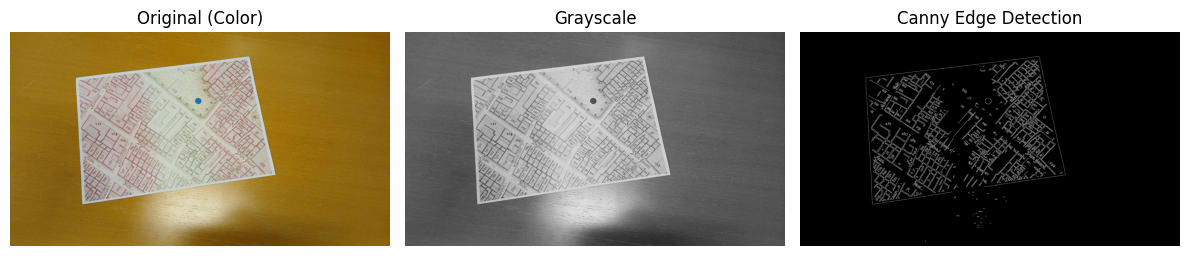
\includegraphics[width=0.9\textwidth]{pics/a7-1.2.png}
    \caption{Canny Edge Detection}
    \label{1.2}
\end{figure}

\begin{lstlisting}
###image load part omitted

image_rgb = cv2.cvtColor(image, cv2.COLOR_BGR2RGB)
image_gray = cv2.cvtColor(image, cv2.COLOR_BGR2GRAY)

image_blur = cv2.GaussianBlur(image_gray, (5, 5), 1.0)

edges = cv2.Canny(image_blur, threshold1=100, threshold2=200)

###Figure Drawing part omitted
\end{lstlisting}
From the result images shown in Figure \ref{1.2}, we can see that the Canny edge detector successfully captures the line structures of the map. The edges of the map and the internal street network are clearly visible. The background area is mostly ignored, and the overall edge detection result appears clean and focused on important structures. This makes Canny especially suitable for analyzing the structure of map-like images.

Compared to Otsu thresholding, Canny does not provide a full foreground region. Instead, it only detects the edges, so it cannot directly generate a region mask. However, for images with complex structures and rich textures, like maps, Canny is very effective at extracting meaningful shapes and lines. If full region segmentation is needed, Canny must be combined with other methods, such as region filling or morphological operations.

In terms of performance, Canny is better at detecting edge outlines, while Otsu is better at separating full regions. When the lighting in an image is uneven, Otsu can mistakenly classify shadows as part of the foreground. In contrast, Canny is more robust to such lighting changes and produces cleaner results.

Canny has several advantages. It can clearly extract structural outlines and is less sensitive to intensity changes such as shadows. It works well for images with line patterns and rich textures. However, it also has some limitations. Canny only gives edge lines, not complete regions. It is also sensitive to noise, which may cause broken edges. Therefore, it is not ideal for tasks that require region masks. Depending on the specific task, Canny and thresholding methods like Otsu can be used together to complement each other.


\section{Image Transform}
%shuangcheng
\subsection{}
\begin{figure}[ht]
    \centering
    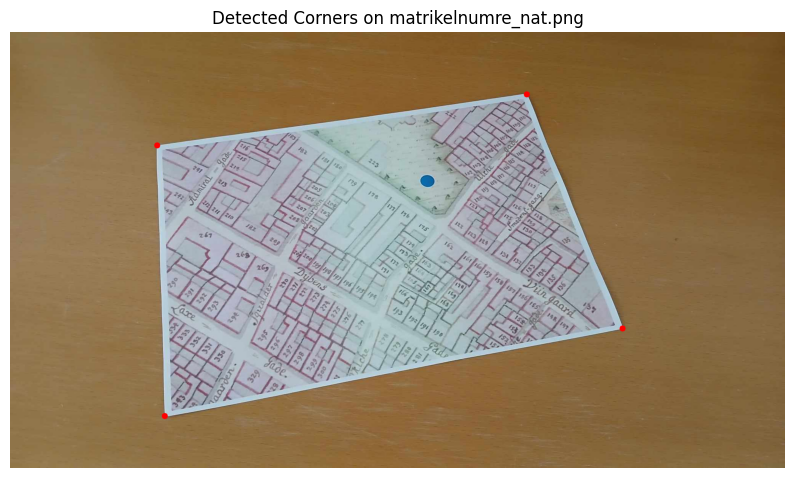
\includegraphics[width=0.7\textwidth]{pics/a7-2.1.png}
    \caption{Corners Detecting}
    \label{2.1}
\end{figure}

\begin{lstlisting}
# Preprocessing: blur + threshold to suppress inner map textures
blurred = cv2.GaussianBlur(gray, (7, 7), 0)
_, thresh = cv2.threshold(blurred, 150, 255, cv2.THRESH_BINARY)

#further denoising using morphological opening
kernel = np.ones((5, 5), np.uint8)
opened = cv2.morphologyEx(thresh, cv2.MORPH_OPEN, kernel)

# Harris corner detection
gray_float = np.float32(opened)
dst = cv2.cornerHarris(gray_float, blockSize=2, ksize=3, k=0.04)

# Dilate corner response to enhance visibility
dst_dilated = cv2.dilate(dst, None)

# Extract corner coordinates using a threshold
corner_threshold = 0.01 * dst_dilated.max()
corner_coords = np.argwhere(dst_dilated > corner_threshold)
corner_coords = np.flip(corner_coords, axis=1)  # Convert to (x, y)

# Find the largest external contour (assumed to be the map border)
contours, _ = cv2.findContours(thresh, cv2.RETR_EXTERNAL, cv2.CHAIN_APPROX_SIMPLE)
largest_contour = max(contours, key=cv2.contourArea)
epsilon = 0.05 * cv2.arcLength(largest_contour, True)
approx_corners = cv2.approxPolyDP(largest_contour, epsilon, True)

# Extract the four corner points
four_corners = [tuple(pt[0]) for pt in approx_corners]

\end{lstlisting}

To reduce the number of irrelevant corner points detected by the Harris algorithm inside the map area, I applied several preprocessing steps to emphasize the paper boundaries and suppress internal details.

First, a Gaussian blur was applied to the image to smooth out fine details. This helped reduce the response to internal lines and lowered their impact on corner detection. Then, a fixed threshold was used to binarize the image, clearly separating the map region from the background and making the paper area stand out. After that, morphological opening was performed to remove small noise points and simplify the overall structure.

Next, the contours of the paper were extracted using the \texttt{findContours} function. A polygonal approximation was then applied using \texttt{approxPolyDP}, which simplified the detected contour into a quadrilateral. From this shape, the four corner points of the map were obtained.

With these preprocessing steps, the Harris corner detection was effectively limited to the outer corners of the map paper as in Figure \ref{2.1}, while ignoring the complex internal building lines.

The final coordinates of the four corner points of the map (Cartesian coordinates): (1360, 166); (387, 300); (407, 1011);(1612, 781).

\subsection{}
\begin{figure}[ht]
    \centering
    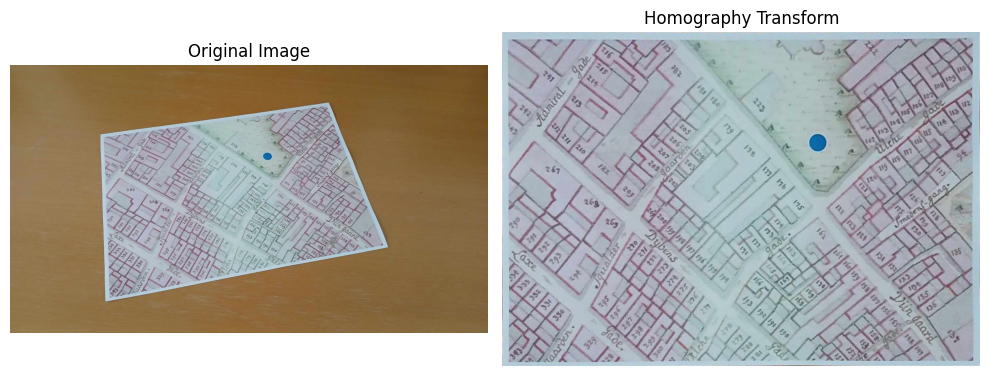
\includegraphics[width=0.7\textwidth]{pics/a7-2.2.png}
    \caption{Homography Transform}
    \label{2.1}
\end{figure}

\begin{lstlisting}
pts_src = np.array([
    [387, 300],     # top-left
    [1360, 166],    # top-right
    [1612, 781],    # bottom-right
    [407, 1011]     # bottom-left
], dtype=np.float32)

width = 1000
height = 700
pts_dst = np.array([
    [0, 0],                 # top-left
    [width - 1, 0],         # top-right
    [width - 1, height - 1],# bottom-right
    [0, height - 1]         # bottom-left
], dtype=np.float32)

H = cv2.getPerspectiveTransform(pts_src, pts_dst)

warped = cv2.warpPerspective(image, H, (width, height))
\end{lstlisting}

To achieve a bird's eye view of the image, we use a homography transformation, which is mathematically defined as:

\[
\begin{bmatrix}
x' \\
y' \\
1
\end{bmatrix}
=
H
\begin{bmatrix}
x \\
y \\
1
\end{bmatrix}
\]

Here, \( H \) is a \( 3 \times 3 \) homography matrix that maps the four corners of the map in the original image to a rectangular region in the target image.

The main steps to achieve that are as follows: we first manually select the four corners of the map in the original image. These points serve as the input points for the transformation. Then, we define the corresponding four corners in the target image, typically forming a regular rectangle. Based on these point pairs, we compute the homography matrix. Finally, we use the \texttt{skimage.transform.warp} function to apply the homography and generate the bird's eye view image.

\section{The Hough Transform}
%zhigao
\subsection{}
\begin{lstlisting}
    def hough_transform(edge_image, theta_step=1, rho_step=1, threshold=100):
    # Chose range and discretization of \rho and \theta.
    rows, cols = edge_image.shape
    diagonal = int(np.ceil(np.sqrt(rows**2 + cols**2)))  # Edge image diagonal length
    thetas = np.deg2rad(np.arange(0, 180, theta_step))   # theta : 0-180 degree
    rhos = np.arange(-diagonal, diagonal, rho_step)      # rho : [-d, d]
    
    # Create accumulator 2D array (Hough Space)
    accumulator = np.zeros((len(rhos), len(thetas)), dtype=np.uint64)
    
    # Iterate over all edge pixels
    edge_points = np.argwhere(edge_image)  # Get all the edge coordinates [y, x]
    
    for (y, x) in edge_points:            # Iterate over each edge point
        for theta_idx, theta in enumerate(thetas):  
            # Calculate the corresponding value of \rho
            rho = x * np.cos(theta) + y * np.sin(theta)
            
            # Ensure that the accumulator array index cannot be negative
            rho_idx = int(round((rho + diagonal) / rho_step))
            
            # Updating the accumulator (to ensure that it does not go out of bounds)
            if 0 <= rho_idx < len(rhos):
                accumulator[rho_idx, theta_idx] += 1
    
    # Lines correspond to accumulator values larger than a certain threshold.
    lines = []
    for rho_idx in range(accumulator.shape[0]):
        for theta_idx in range(accumulator.shape[1]):
            if accumulator[rho_idx, theta_idx] >= threshold:
                lines.append( (rhos[rho_idx], thetas[theta_idx]) )
    
    return lines, accumulator
\end{lstlisting}
The code is written strictly following the steps on slide.
Firstly input the edge image, the step size and the threshold value. Determine the range of $ \theta $ and $ \rho $ according to the steps in slide.
Then the first iteration is performed and the corresponding $ \rho $ is computed. the second iteration gets the lines that are greater than the threshold.


Computational complexity (two iterations): 
\[ O(E \times T) + O(R \times T) \]
E: indicates the number of edge pixels.
T: The number of $ \theta $
R: The number of all calculated $ \rho $ in the accumulator

\subsection{}
\begin{figure}[ht]
    \centering
    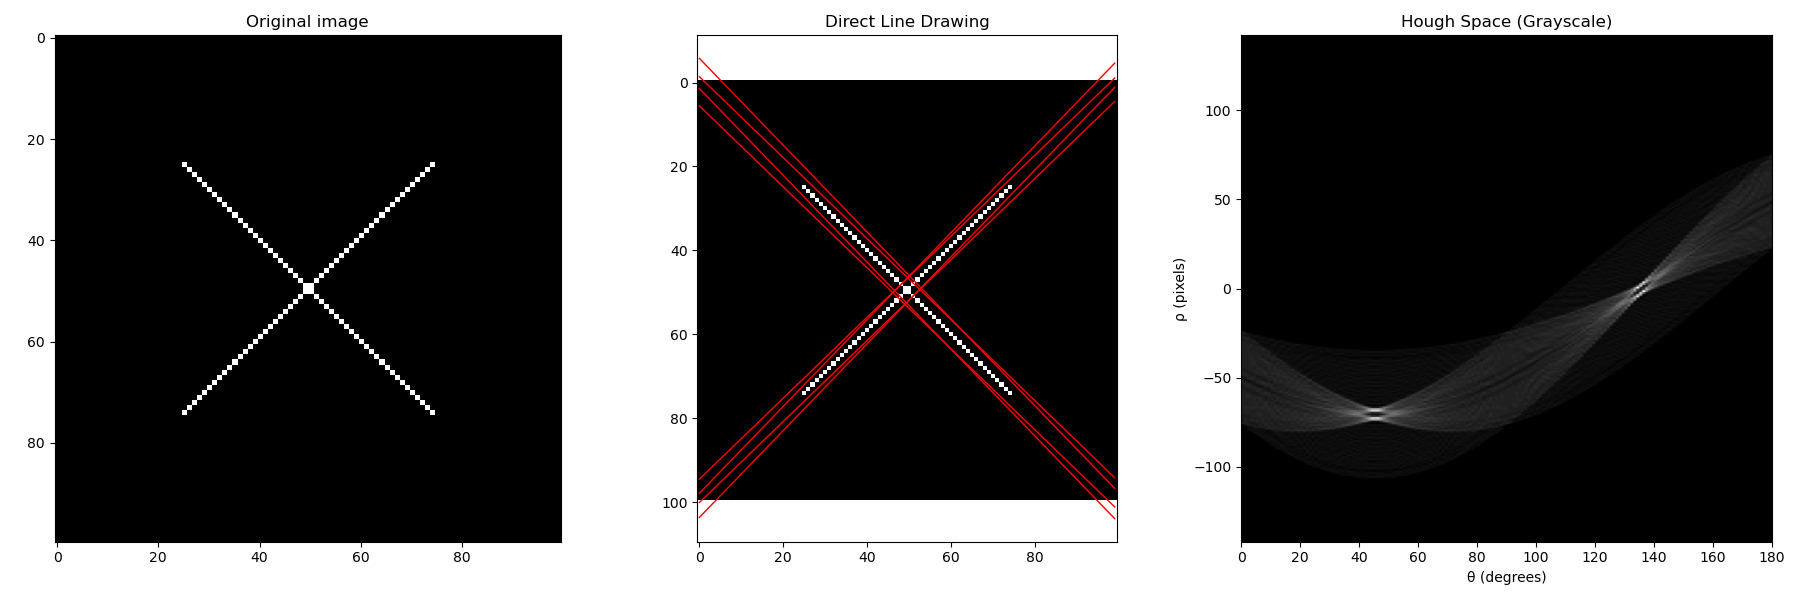
\includegraphics[width=0.7\textwidth]{pics/A7_3.2_1.png} 
    \caption{Hough Transform by my implementation}
    \label{fig: Figure 6}
\end{figure}
\begin{figure}[ht]
    \centering
    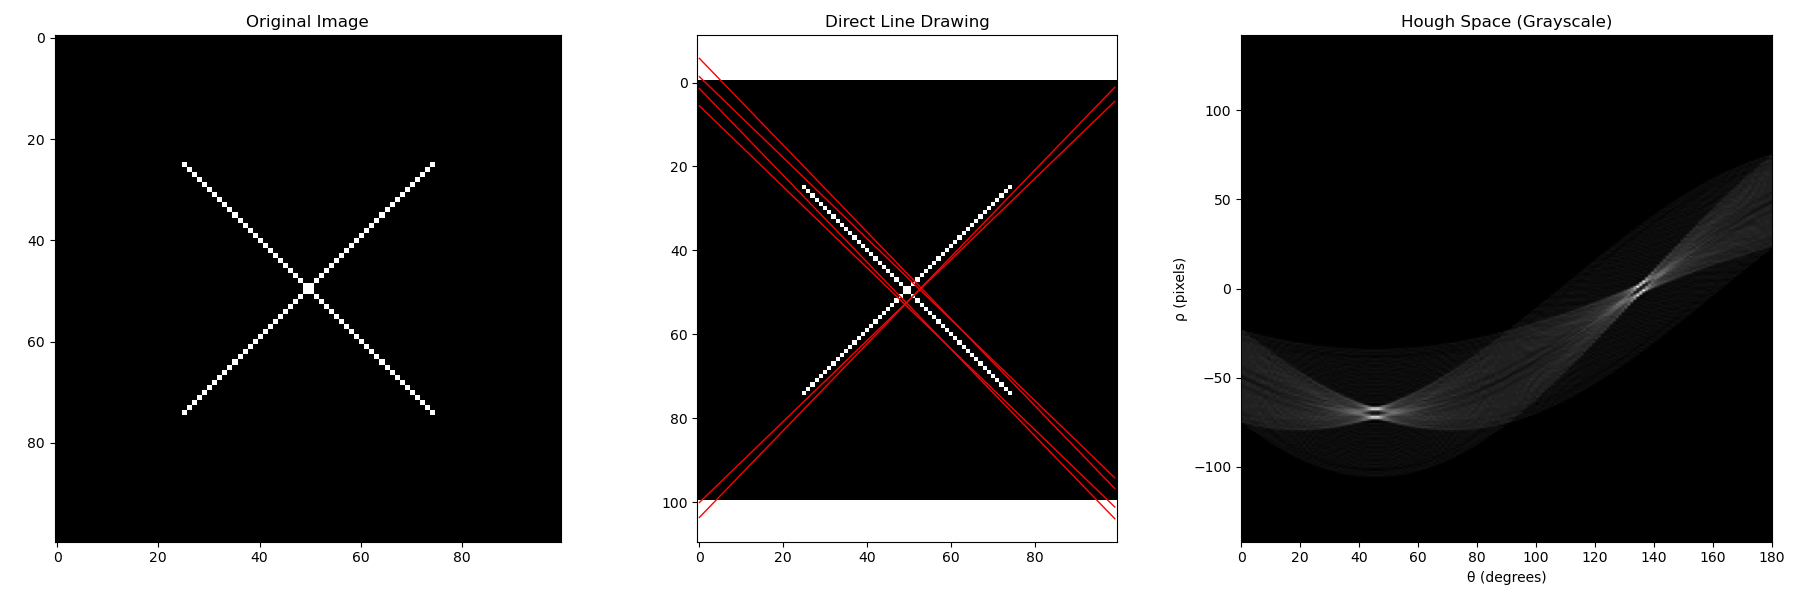
\includegraphics[width=0.7\textwidth]{pics/A7_3.2_2.png} 
    \caption{Hough Transform by skimage}
    \label{fig: Figure 7}
\end{figure}
First of all, my implementation and skimga's implementation output the same Hough transform.
But as can be seen in Figures \ref{fig: Figure 6} and \ref{fig: Figure 7}, my method outputs more lines for the same threshold.
I think there may be a difference in the method of calculation, skimage's method may filter adjacent peaks resulting in fewer lines.
\subsection{}
\begin{figure}[ht]
    \centering
    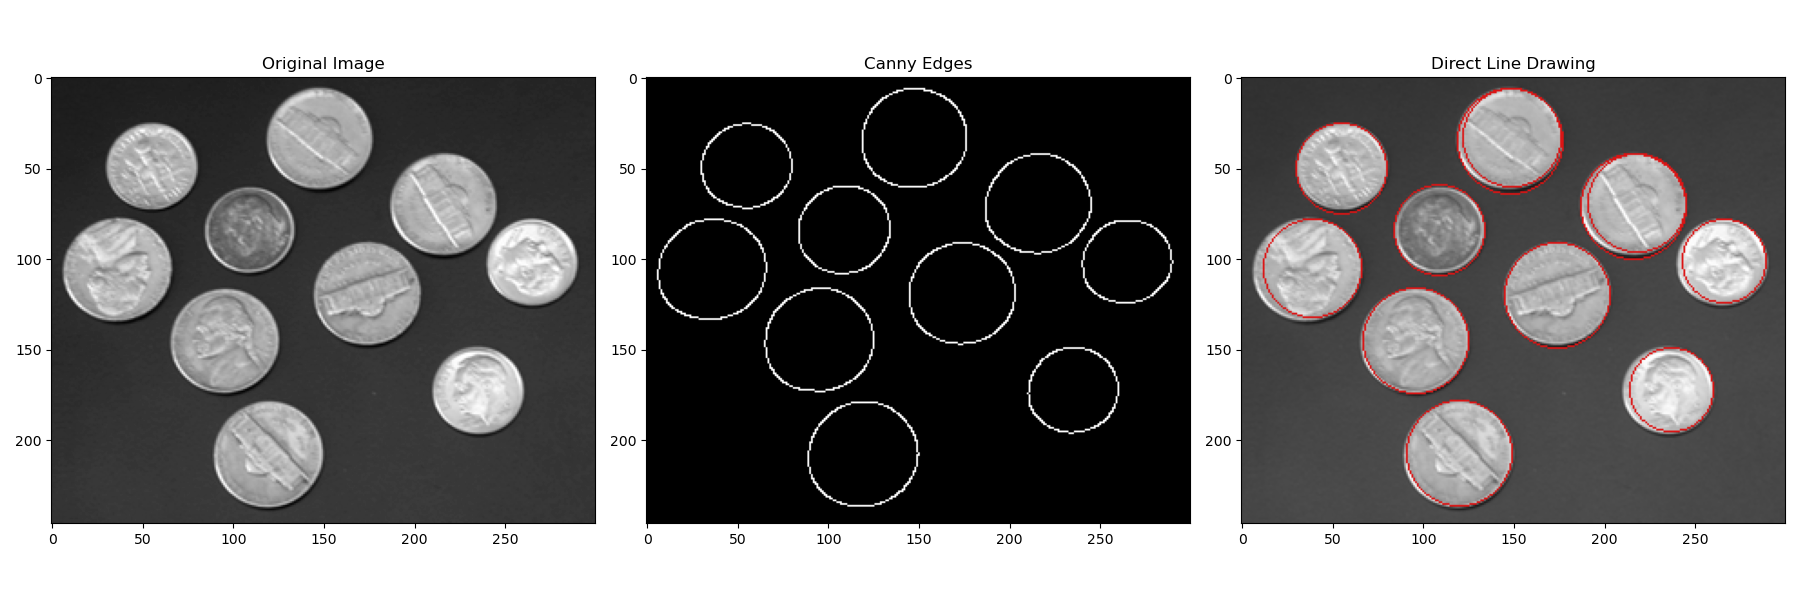
\includegraphics[width=0.8\textwidth]{pics/A7_3.3.png} 
    \caption{Hough circle by skimage}
    \label{fig: Figure 8}
\end{figure}
First use the Canny method to get the edge graph.
Then set a radius range, based on the size of the coin in the picture. 
The next step is to call the hough-circle method to get the accumulator, and finally call hough-circle-peaks to get the most obvious circle and draw it.
Figure \ref{fig: Figure 8} shows the final result.

\newpage
\subsection{}
\begin{lstlisting}
import numpy as np
import matplotlib.pyplot as plt
from skimage import io, color, morphology, feature, transform

# Grayscale image conversion.
image = io.imread('transformed_map.png')
image = image[..., :3]
gray = color.rgb2gray(image)

# Canny edge image generation
edges = feature.canny(gray, sigma=2)

# Setting radius intervals and detecting circles
radii = np.arange(7, 10, 1) 
hough_res = transform.hough_circle(edges, radii)
accums, cx, cy, radii = transform.hough_circle_peaks(
    hough_res, radii, total_num_peaks=1
)

\end{lstlisting}
\begin{figure}[ht]
    \centering
    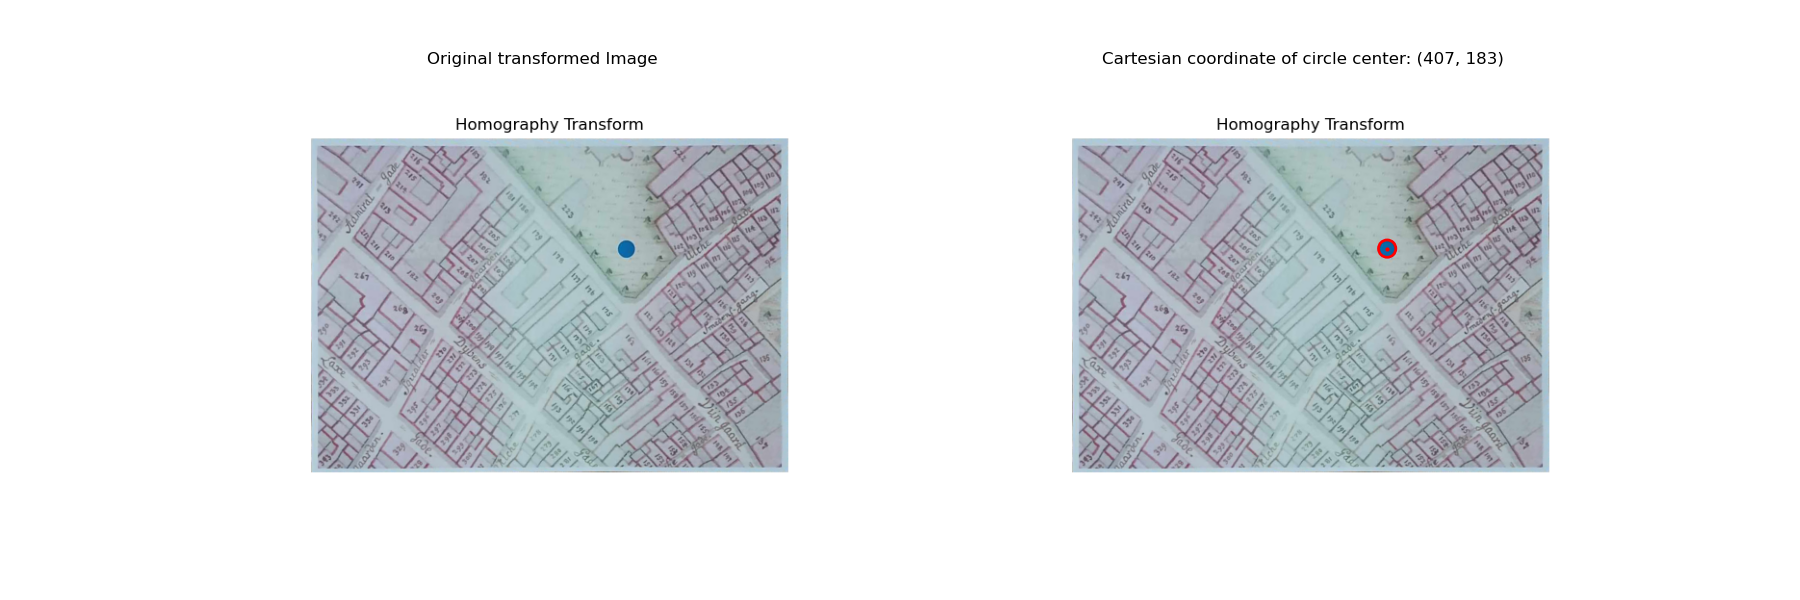
\includegraphics[width=1\textwidth]{pics/A7_3.4.png} 
    \caption{Bird’s eye view transformed map and draw of circle}
    \label{fig: Figure 9}
\end{figure}
Firstly the edge image is got using Canny method. Then using hough\_circle, a Hough accumulator is generated.
The Hough Circle Transform actually finds the combination of circle parameters corresponding to each edge point of the edge image, i.e., the circle centre coordinates and radius. The parameter combinations are then voted on and the high vote regions correspond to the possible circles.
Finally use the hough\_circle\_peaks method to get the peaks, which are the circle parameters.
\section{Morphology}
%wanjing
\subsection{} % 4.1

\subsubsection{Applying Opening and Closing} % 4.1.1 

Figure~\ref{fig:full_images} \textit{Original} shows the original image, as well as the results of the opening and closing operations in \textit{Opened} and \textit{Closed} (Here we choose disk=1). A zoomed-in region is presented in Figure~\ref{fig:full_images} \textit{Zoom}, \textit{Opened Zoom} and \textit{Closed Zoom} to highlight local changes.

\textbf{Changes: } As shown in the space around largest white spot, the \textit{Opened} removes small white specks and breaks thin connections, and the \textit{Closed} fills small black holes and merges nearby regions.

\begin{figure}[ht]
    \centering
        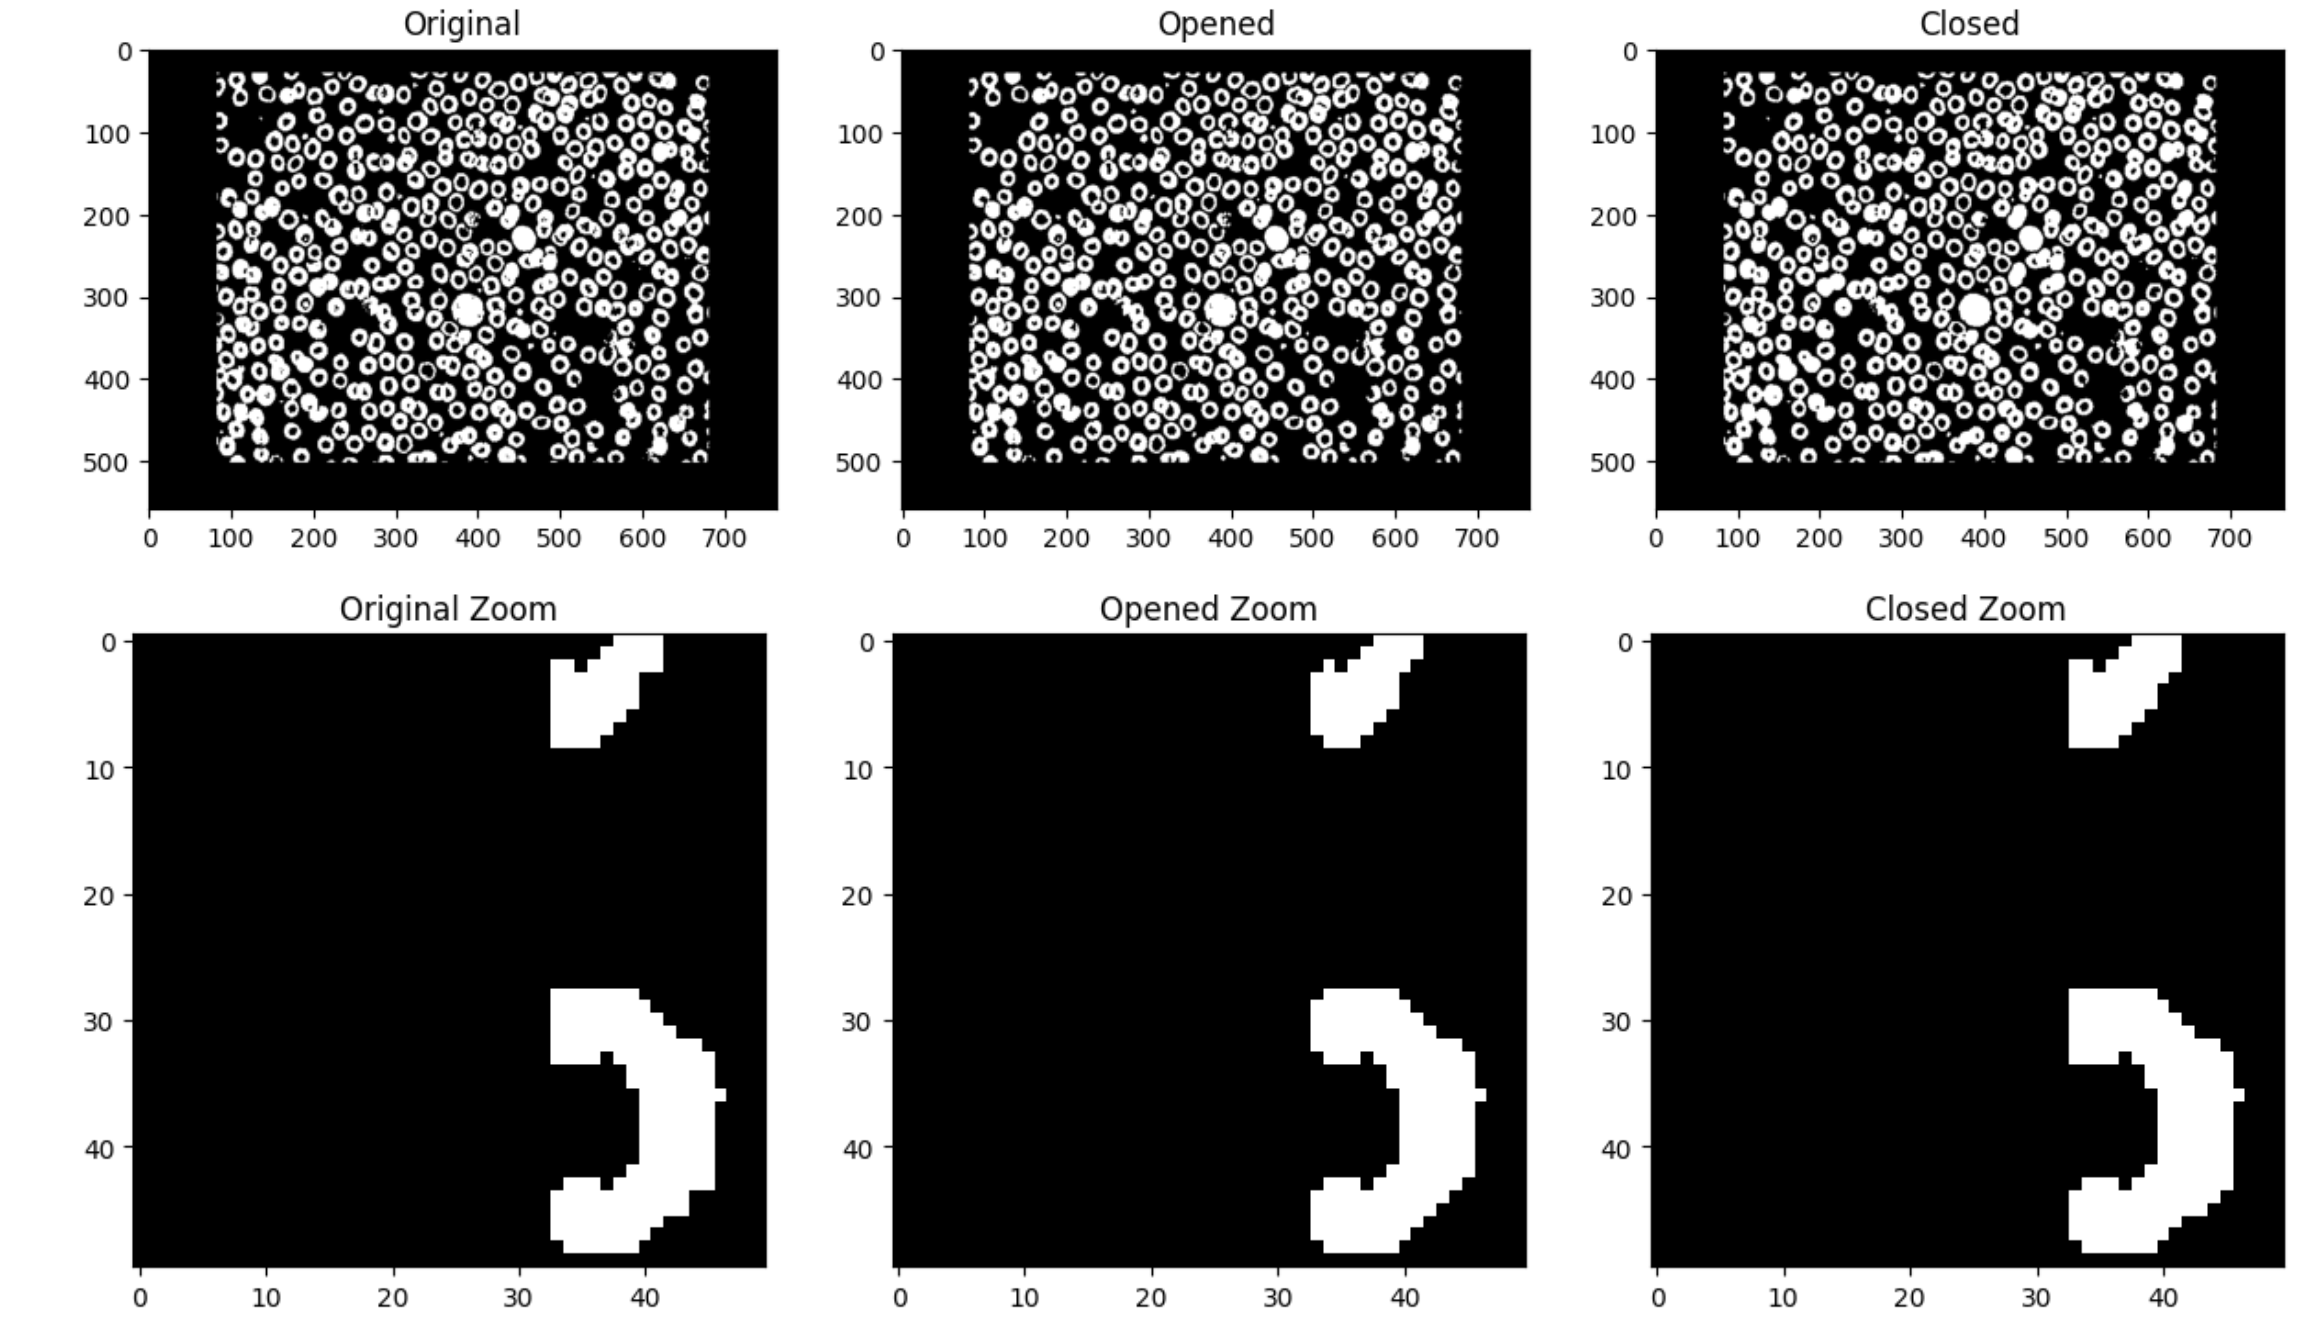
\includegraphics[width=0.9\textwidth]{pics/a7-4.1.1}
    \caption{Original and Morphologically Processed Images}
    \label{fig:full_images}
\end{figure}


\subsubsection{Differences and Challenges} % 4.1.2 
\textbf{A. } As noted in the course material \textit{Mathematical morphology - properties of dilation and erosion} page 17, opening and closing are dual operations; opening erodes then dilates (removing small bright objects), while closing dilates then erodes (filling small dark holes). In this case, opening reduces small cell fragments and isolates larger structures, whereas closing connects adjacent components and fills gaps.

\textbf{B. } When separating individual cells with those methods, some cells remain connected after closing, making separation difficult, and then opening may remove small structures that are actually part of valid cells. Also, these operations are not sufficient to segment overlapping or touching cells completely.

\subsubsection{Connected Components Analysis} % 4.1.3 

Figure \ref{fig:connected_components} shows the labeled images. For the different connected components, Opened image yields more labels (separated cells) with number=369, and the Closed image has fewer labels (merged cells), indicating over-merging, with number = 343.


\begin{lstlisting}
from skimage.measure import label

# Label connected components
labels_open = label(opened, connectivity=2)
labels_close = label(closed, connectivity=2)

print(f"Opened labels: {labels_open.max()}") # num_opened
print(f"Closed labels: {labels_close.max()}") # num_closed

# Visualize labels
plt.figure(figsize=(10,5))
plt.subplot(121).imshow(labels_open, cmap='nipy_spectral')
plt.title(f'Connected Components (Opened) - {labels_open.max()} labels')
plt.subplot(122).imshow(labels_close, cmap='nipy_spectral')
plt.title(f'Connected Components (Closed) - {labels_close.max()} labels')
plt.show()
\end{lstlisting}


\begin{figure}[ht]
    \centering
        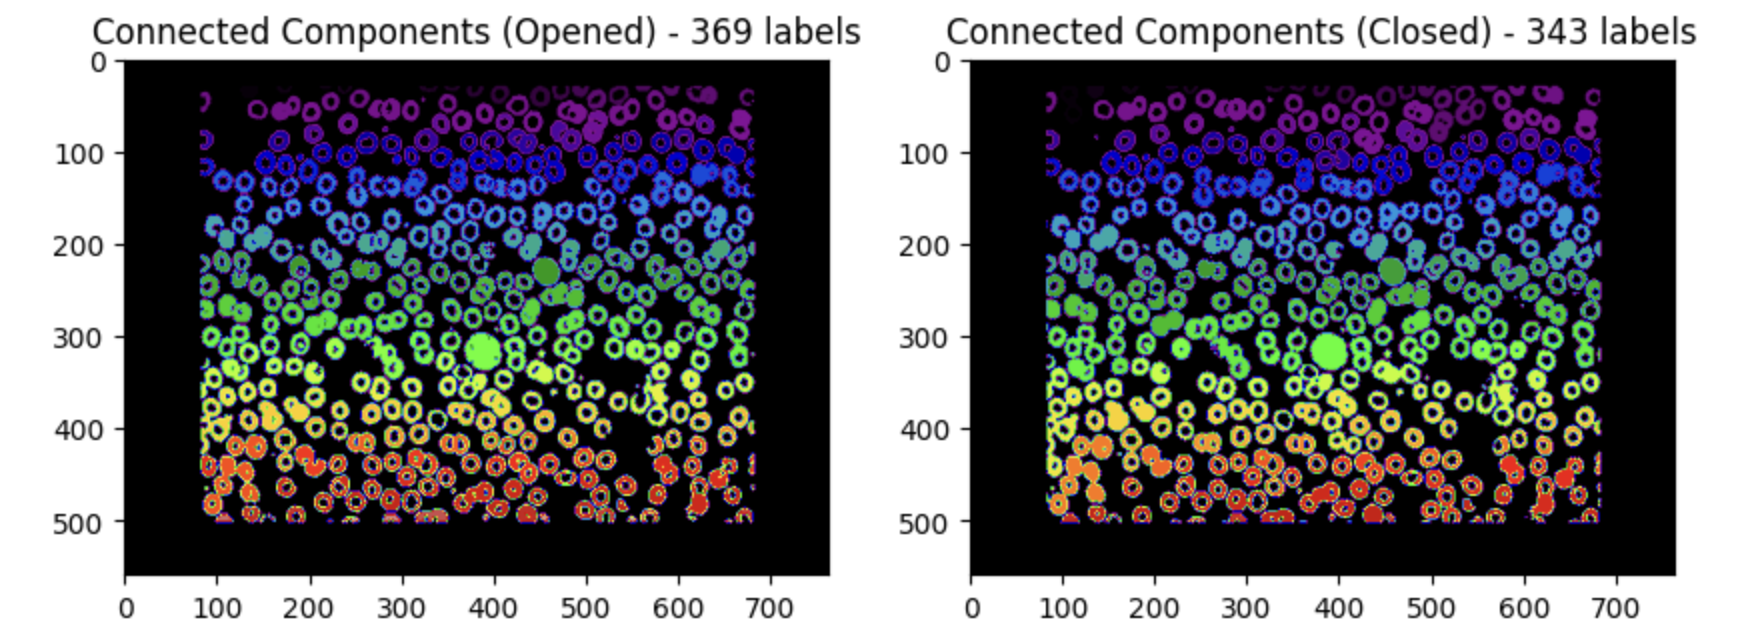
\includegraphics[width=\textwidth]{pics/a7-4.1.3}
    \caption{Connected Component Labeling Results}
    \label{fig:connected_components}
\end{figure}

\textbf{Reflection: }We find the opening operation tends to break apart connected cells, increasing the number of detected components. The closing operation joins adjacent cells, reducing the total number of detected components. Also, neither operation is fully effective at isolating individual cells, and additional techniques such as watershed segmentation may be required.

\subsection{} % 4.2

Final total amount 45 kr. What we did: First we convert he input image to a binary format by setting pixels above a certain intensity threshold to \texttt{True}. 
Then we apply Morphological Closing. The small gaps in the binary image are filled using a disk-shaped structuring element of radius 5.

Then we did Connected Component Analysis. we use the \texttt{measure.label} function and it identifies individual objects (coins) in the image using 8-connectivity.

Then we compute the Region Properties with function \texttt{measure.regionprops\_table}. It computes the area of each labeled region.

Finally the coins are assigned a denomination based on their area, and we sum up the assigned values as the total amount. Our rules of the mapping the areas to values is as follows:
    \begin{itemize}
        \item If area $> 1000$, assign 20 kr.
        \item If area $> 500$, assign 10 kr.
        \item Otherwise, assign 5 kr.
    \end{itemize}

\subsection{} % 4.3

After both trying out opening and closing, we choose the \textit{Closing (Dilation + Erosion)} to fill thin black lines (0s in the binary mask) while preserving the shape of larger structures (map outline and blue dot). The disk-shaped structuring element ensures isotropic processing to handle lines in any direction.

After trying different parameters(disk radius=1,2,3,4,5), we choose the disk of radius 2, and it is large enough to cover the thickness of the lines but small enough to avoid distorting critical features.

\begin{lstlisting}
# Define different structuring element sizes
disk_sizes = [1, 2, 3, 4, 5]

fig, axes = plt.subplots(len(disk_sizes), 3, figsize=(15, 10))

for i, size in enumerate(disk_sizes):
    selem = morphology.disk(size)

    # Perform opening and closing
    opened = morphology.opening(binary_nat, selem)
    closed = morphology.closing(binary_nat, selem)

    # Plot original, opened, and closed images
    axes[i, 0].imshow(binary_nat, cmap='gray')
    axes[i, 0].set_title(f'Original (Disk={size})')

    axes[i, 1].imshow(opened, cmap='gray')
    axes[i, 1].set_title(f'Opened (Disk={size})')

    axes[i, 2].imshow(closed, cmap='gray')
    axes[i, 2].set_title(f'Closed (Disk={size})')

plt.tight_layout()
plt.show()
\end{lstlisting}

For the result visualization, we overlay the original binary image and cleaned result and high light the difference, as shown in Figure~\ref{fig:viz}.

\begin{figure}[ht]
    \centering
        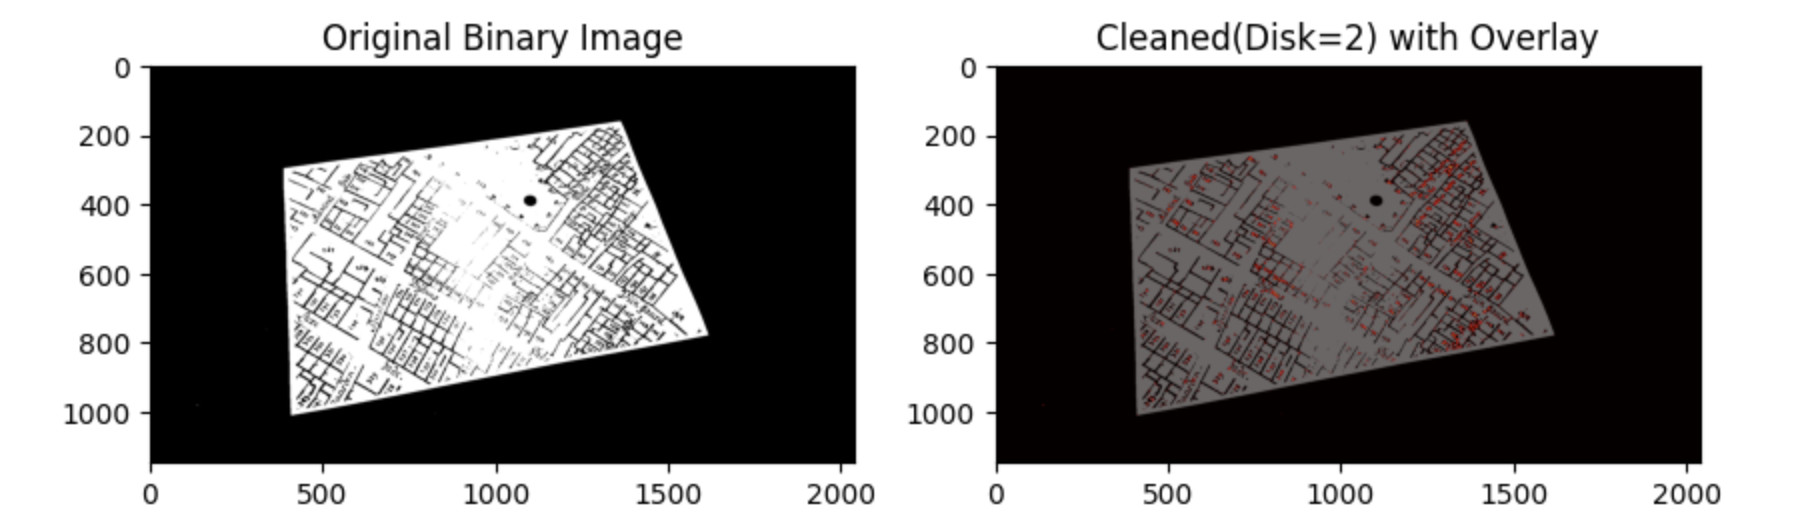
\includegraphics[width=\textwidth]{pics/a7-4.3}
    \caption{Visualization of the cleaned binary segmentation mask}
    \label{fig:viz}
\end{figure}


\end{document}
